\documentclass{../source/zjureport}

\major{信息工程}
\name{周灿松}
\title{实验设计报告}
\stuid{3190105055}
\college{信息与电子工程学院}
\date{\today}
\lab{教11-400}
\course{计算机组成与设计}
\instructor{屈民军、唐奕}
\grades{}
\expname{实验设计报告}
\exptype{设计实验}
\partner{}

\begin{document}
    \makecover
    \makeheader

    \section{实验步骤}
    \begin{enumerate}
        \item 根据书中四位先行进位加法器的设计方案完成四位先行进位加法器的设计,并对其进行功能仿真
        \item 编写有条件的加法器结构(CSA_4.v),为后续搭建32位快速加法器做好准备工作
        \item 对32位快速加法器进行功能仿真与时序仿真,分析仿真结果
    \end{enumerate}

    \section{实验数据记录与分析}
        \subsection{4位先行进位加法器}
            \subsubsection{仿真图像}
                \begin{figure}[!htp]
                    \centering
                    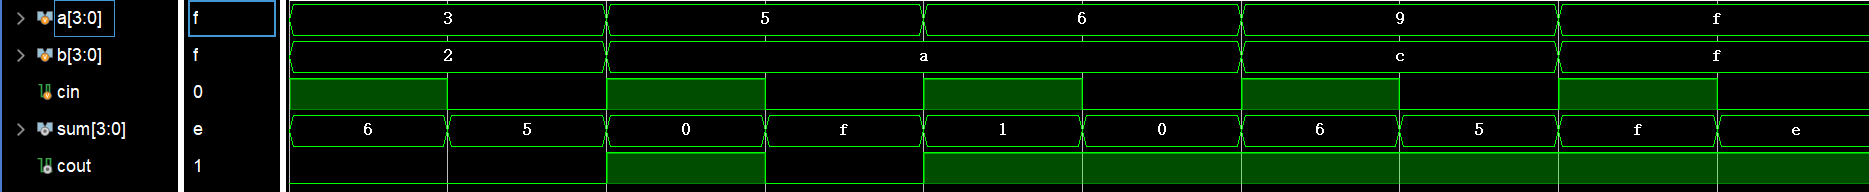
\includegraphics[width = 0.8\textwidth]{figure/adder_4bits.png}
                    \caption{四位先行进位加法器仿真}
                \end{figure}
            \subsubsection{结果分析}
            观察图像可以发现:当a+b+ci>=f时,cout=1,s = a+b+ci-f;其余情况下cout=0,s=a+b+ci;

            由此可以得出结论,4位先行进位加法器运行正常。
        \subsection{32位进位选择加法器}
            \subsubsection{功能仿真结果}
                \begin{figure}[!htp]
                    \centering
                    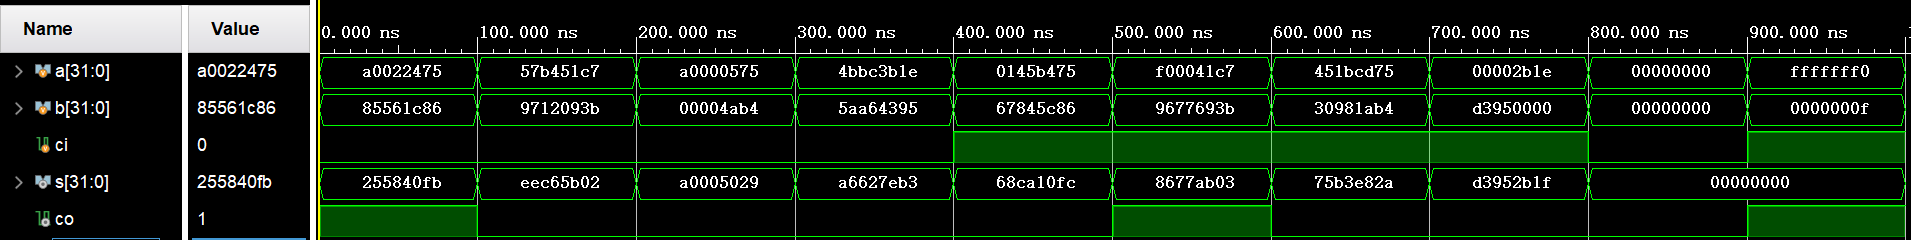
\includegraphics[width = 0.8\textwidth]{figure/behaviorSimulation1.png}
                    \caption{功能仿真结果}
                \end{figure}
            \subsubsection{时序仿真结果}
                \begin{figure}[!htp]
                    \centering
                    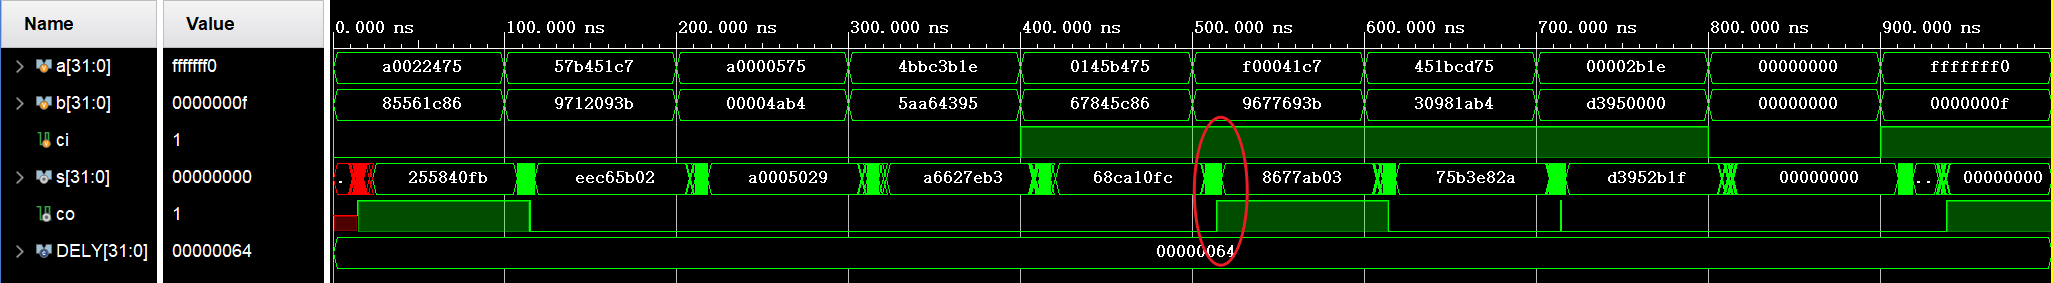
\includegraphics[width = 0.8\textwidth]{figure/timingSimulation.png}
                    \caption{时序仿真结果}
                \end{figure}
            \subsubsection{结果分析}
                因为加法器为32位加法器,所以当结果超过了0xffff_ffff后会产生一个
                进位信号,也就是co=1,而s中存储的则是结果的低32位。利用计算器
                对波形进行验证,可以发现所有的测试样例均符合上诉结论,所以可以得出
                32位进位选择加法器结果运行结果正常。

                而在时序仿真中,除去功能仿真中的结论,还反映出了信号的时延。观察红
                圈中的波形,我们可以发现进位信号co先于结果s出现,这一结果产生也是
                符合预期的:
                
                因为在四位先行进位加法器中,会先行计算出$G_i$与$P_i$,这
                是第一级时延,然后会利用产生的$G_i$与$P_i$生成进位信号$C_i$,这是第二
                级时延,最后$S$则是在进位信号产生后再出现。所以在时序仿真结果中,进位信号
                会先于结果信号出现在波形之中。

                由上述分析可以得出结果:此32位进位选择加法器功能正常。

    \section{思考题}
        \subsection{为什么要进行时序仿真?}
        时序仿真利用综合实现后的连线信息以及时延信息,在最坏的情况下对电路的时延进行评估。这种
        分析是非常有必要的,它能够验证我们设计的电路是否符合时延要求,相比功能仿真更加能够反映
        电路的性能。

    \section{心得体会}
        因为本次实验是后续CPU设计的热身实验,所以整体上难度不是特别大,代码实现以及仿真结果分析
        都比较简单。不过这次实验也让我第一次接触到了时序仿真,这应该算是最大的收获了。

        除此以外,在本次实验中我试着全程使用vivado自带的仿真器,相较于modelsim,vivado自带的
        仿真器用着体验好了不少,主要体现在仿真操作比modelsim更加地简单便捷。

\end{document}